\section{构建小轮组三维模型}
\begin{procedure}
\item 初始化绘图环境

\begin{enumerate}
\item 新建带国家标准标注样式的文件。

以带标国家标准标注样式的样板文件“GBacadiso”为样板创建新的AutoCAD绘图文件。

\item 切换至西南等轴测图。

\begin{lstlisting}
命令: -VIEW
输入选项 [?/删除(D)/正交(O)/恢复(R)/保存(S)/设置(E)/窗口(W)]: swiso
\end{lstlisting}

\item 定义用户坐标系,使其$xy$平面与左视图投影面平行。

由于小轮组的组成零件中大多数的回转体特征面与左视图投影面平行,因此本例选择将用户坐标系定义为与左视图投影面平行。当然也可以不进行此操作,只是显示结果与本例会略有差异,但操作过程是基本一致的。

\begin{lstlisting}
命令: UCS
当前 UCS 名称: *世界*
指定 UCS 的原点或 [面(F)/命名(NA)/对象(OB)/上一个(P)/视图(V)/世界(W)/X/Y/Z/Z 轴(ZA)] <世界>: za
指定新原点或 [对象(O)] <0,0,0>:
在正 Z 轴范围上指定点 <0.0000,0.0000,1.0000>: -1,0,0
\end{lstlisting}
\end{enumerate}

\item 复制小轮组组件三维模型

用AutoCAD打开之前建立好的轮零件三维模型文件,调出轮零件的三维模型。为实现将轮零件的三维模型复制到新建的AutoCAD文件之中,需要先将轮零件的三维模型先复制来剪切板之中,然后再将其粘粘贴到新建到的AutoCAD文件之中。通常实现将AutoCAD对象复制到剪切板的方法有:
\begin{itemize}
\item 键盘输入copyclip\index{copyclip,复制到剪切板}
\item 
\includegraphics[scale=0.3]{keyctrl}+
\includegraphics[scale=0.3]{keyc}
\item 【编辑】$\rightarrow $【复制】
\item 【标准】
\includegraphics[scale=0.45]{biaozhuntools}工具栏中的
\includegraphics[scale=0.45]{copyclip}图标
\end{itemize}

命令调用后选择轮零件的三维模型并结束选择即可将其复制到剪切板之中。
\begin{lstlisting}
命令: COPYCLIP
选择对象: 找到 1 个
选择对象:
\end{lstlisting}

接下来进入新建的AutoCAD文件之中,调用粘贴命令来实现将剪切板中的轮零件三维模型复制到文件之中。通常调用粘贴命令的方法有:
\begin{itemize}
\item 键盘输入pasteclip\index{pasteclip,粘贴自剪切板}
\item 
\includegraphics[scale=0.3]{keyctrl}+
\includegraphics[scale=0.3]{keyv}
\item 【编辑】$\rightarrow $【粘贴】
\item 【标准】
\includegraphics[scale=0.45]{biaozhuntools}工具栏中的
\includegraphics[scale=0.45]{pasteclip}图标
\end{itemize}

命令调用后,在绘图区中任意选取一点作为插入点,即可完成轮零件三维的模型的复制,结果如图\ref{fig:xiaolunzhuangpei1} 所示。
\begin{lstlisting}
命令:  PASTECLIP
指定插入点:
\end{lstlisting}


\begin{figure}[htbp]
\centering
\subfloat[]{\label{fig:xiaolunzhuangpei1}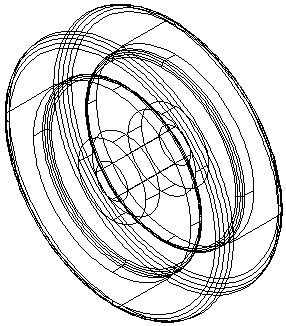
\includegraphics[scale=0.4]{xiaolunzhuangpei1}}\hspace{20pt}
\subfloat[]{\label{fig:xiaolunzhuangpei2}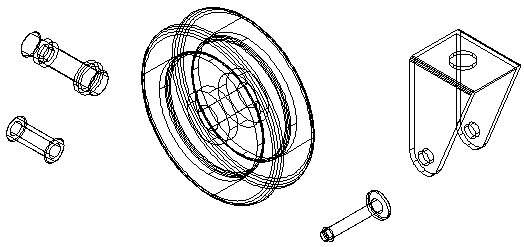
\includegraphics[scale=0.5]{xiaolunzhuangpei2}}
\caption{复制小轮组组成零件}
\end{figure}

按照上述方法依次将小轮组的其它零件复制过来,结果如图\ref{fig:xiaolunzhuangpei2}所示。
\item 组装套筒与轮

在实际生产之中零件的装配是有先后顺序的。如果顺序错误是无法完的成部件的组装的。尽管在AutoCAD中不依照生产实际的顺序任然能够构建部件的三维装配模型,但是遵循生产实际的装配顺序能够有助于我们更深入地理解装配图的作用。在此,我们先将套筒和轮装配在一起。通过观察图\ref{fig:xiaolunzhuangpei2}可知,套筒的轴心线与轮孔的轴心线不是相互平行的,因此无法直接用移动命令来完成组装操作。一种可行的方法是:先将笔筒旋转至与轮轴心线平行的位置,然后再通过移动来完成操作。但是AutoCAD中还有更为方便的命令——三维对齐可以直接完成此项任务,其调用方法有:
\begin{itemize}
\item 键盘输入3dalign\index{3dalign,三维对齐}
\item 【修改】$\rightarrow $【三维操作】$\rightarrow $【三维对齐】
\item 【建模】
\includegraphics[scale=0.45]{solidtoolbar}工具栏中的【三维对齐】
\includegraphics[scale=0.45]{3dalign}
\end{itemize}

\begin{figure}[htbp]
\centering
\subfloat[]{\label{fig:3dalignselect}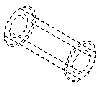
\includegraphics[scale=1]{3dalignselect}}\hspace{20pt}
\subfloat[]{\label{fig:3dalignselect1}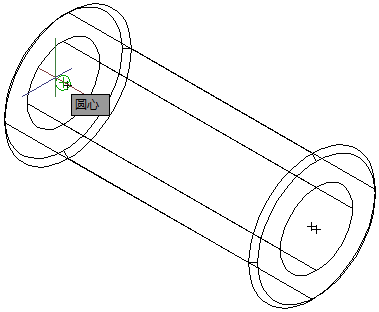
\includegraphics[scale=0.3]{3dalignselect1}}\\
\subfloat[]{\label{fig:3dalignselect2}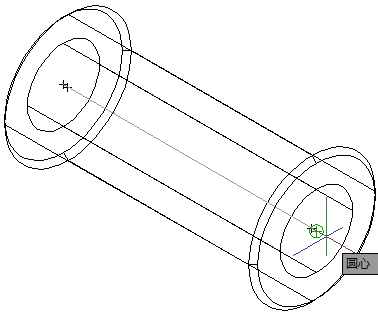
\includegraphics[scale=0.3]{3dalignselect2}}\hspace{20pt}
\subfloat[]{\label{fig:3dalignselect3}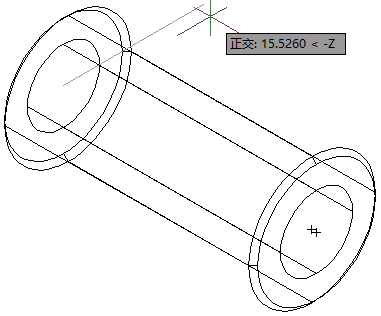
\includegraphics[scale=0.3]{3dalignselect3}}
\caption{三维对齐操作过程(一)}
\end{figure}

三维对齐命令调用后选择套筒作为要对齐的对象,选择后会以虚线的形式予以标识,效果如图\ref{fig:3dalignselect}所示。
\begin{lstlisting}
命令: 3DALIGN
选择对象: 找到 1 个
选择对象:
\end{lstlisting}

接下来是指定源平面和方向,为方便操作应向上轻推鼠标滚轮将套筒零件模型进行适当的放大,选择图\ref{fig:3dalignselect1}所示的圆心作为基点,选择图\ref{fig:3dalignselect2}所示的圆心作为第二个点,为方便选择与套筒轴心线垂直的点,用
\includegraphics[scale=0.3]{keyf8}键开启正交模式,并以图\ref{fig:3dalignselect3}的方式选择第三点。
\begin{lstlisting}
 指定源平面和方向 ...
指定基点或 [复制(C)]:
指定第二个点或 [继续(C)] <C>:
指定第三个点或 [继续(C)] <C>:
\end{lstlisting}

\begin{figure}[htbp]
\centering
\subfloat[]{\label{fig:3dalignselect4}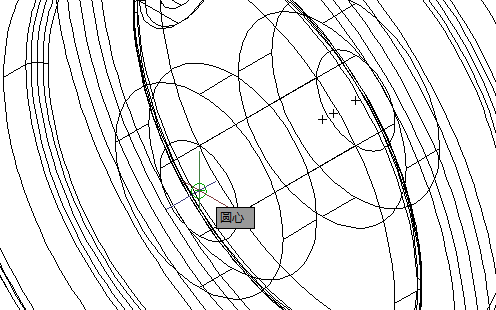
\includegraphics[scale=0.3]{3dalignselect4}}\hspace{20pt}
\subfloat[]{\label{fig:3dalignselect5}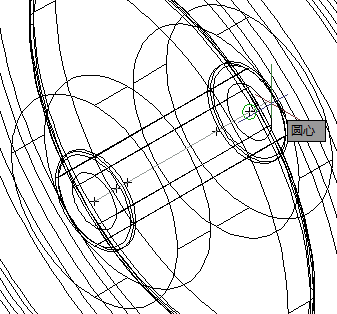
\includegraphics[scale=0.3]{3dalignselect5}}\hspace{20pt}
\subfloat[]{\label{fig:xiaolunzhuangpei3}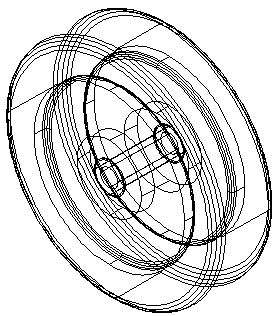
\includegraphics[scale=0.3]{xiaolunzhuangpei3}}
\caption{三维对齐操作过程(二)}
\end{figure}

接下来指定目标平面和方向,按图\ref{fig:3dalignselect4}所示选择轮零件模型上的圆心作为第一个目标点,选择图\ref{fig:3dalignselect5}的圆心作为每个目标点,并以正交模式任意指定一个与轴线垂直的点作为第三个目标点,对齐后的效果如图\ref{fig:xiaolunzhuangpei3} 所示。
\begin{lstlisting}
 指定目标平面和方向 ...
指定第一个目标点:
指定第二个目标点或 [退出(X)] <X>:
指定第三个目标点或 [退出(X)] <X>:
指定第三个目标点或 [退出(X)] <X>:
\end{lstlisting}

\item 组装支架与连接杆

完成套筒与轮的组装后,需要将支架与连接杆组装在一起,任然使用三维对齐命令来完成。组装完成后效果如图\ref{fig:xiaolunzhuangpei4}所示。
\begin{lstlisting}
命令: 3DALIGN
选择对象: 找到 1 个
选择对象:
 指定源平面和方向 ...
指定基点或 [复制(C)]:
指定第二个点或 [继续(C)] <C>:
指定第三个点或 [继续(C)] <C>:
 指定目标平面和方向 ...
指定第一个目标点:
指定第二个目标点或 [退出(X)] <X>:
指定第三个目标点或 [退出(X)] <X>:
指定第三个目标点或 [退出(X)] <X>:
\end{lstlisting}

\begin{figure}[htbp]
\centering
\begin{floatrow}[3]
\ffigbox{\caption{组装支架与连接杆}\label{fig:xiaolunzhuangpei4}}{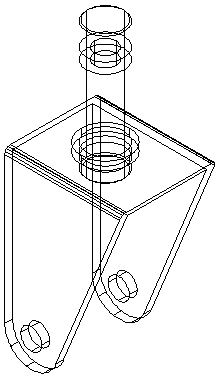
\includegraphics[scale=0.3]{xiaolunzhuangpei4}}
\ffigbox{\caption{支架辅助轴线}\label{fig:drawaidline1}}{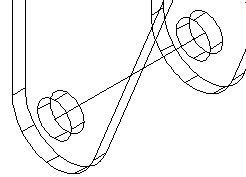
\includegraphics[scale=0.3]{drawaidline1}}
\ffigbox{\caption{套筒辅助轴线}\label{fig:drawaidline2}}{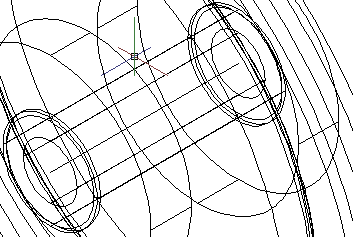
\includegraphics[scale=0.3]{drawaidline2}}
\end{floatrow}
\end{figure}
\item 组装套筒轮组件与支架连杆组件

为方便将套筒和轮构成组件定位于支架安装孔的正中位置,需要先绘制辅助线。首先绘制支架的辅助线,结果如图\ref{fig:drawaidline1}所示。
\begin{lstlisting}
命令: line
指定第一个点:
指定下一点或 [放弃(U)]:
指定下一点或 [放弃(U)]:
\end{lstlisting}

接下来绘制套筒的辅助线,结果如图\ref{fig:drawaidline2}所示。
\begin{lstlisting}
命令: line
指定第一个点:
指定下一点或 [放弃(U)]:
指定下一点或 [放弃(U)]:
\end{lstlisting}

用移动命令来实现两个组件的组装。即同时选择套筒和轮作为移动对象,选择套筒辅助线的中点作为基点,选择支架辅助线的中点作为第二个点。完成后的效果如图\ref{fig:xiaolunzhuangpei5}所示。

\begin{lstlisting}
命令: move
选择对象: 指定对角点: 找到 3 个
选择对象:
指定基点或 [位移(D)] <位移>:
指定第二个点或 <使用第一个点作为位移>:  
\end{lstlisting}
\begin{figure}[htbp]
\begin{floatrow}[2]
\ffigbox{\caption{套筒轮组件与支架连杆组件组装结果}\label{fig:xiaolunzhuangpei5}}{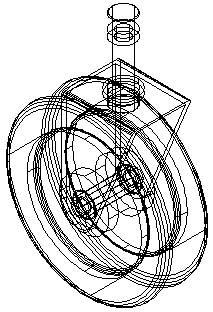
\includegraphics[scale=0.5]{xiaolunzhuangpei5}}
\ffigbox{\caption{小轮组三维模型}\label{fig:xiaolunzhuangpei6}}{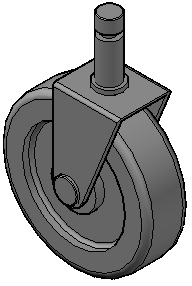
\includegraphics[scale=0.5]{xiaolunzhuangpei6}}
\end{floatrow}
\end{figure}
\item 组装轴

由于轴的轴线与图\ref{fig:xiaolunzhuangpei5}的组件轴心线不平行,因此用三维对齐命令来完成轴的组装。

\begin{lstlisting}
命令: 3DALIGN
选择对象: 找到 1 个
选择对象:
 指定源平面和方向 ...
指定基点或 [复制(C)]:
指定第二个点或 [继续(C)] <C>:
指定第三个点或 [继续(C)] <C>:
 指定目标平面和方向 ...
指定第一个目标点:
指定第二个目标点或 [退出(X)] <X>:
指定第三个目标点或 [退出(X)] <X>:
指定第三个目标点或 [退出(X)] <X>:
\end{lstlisting}

\item 切换视觉样式

为便于观察小轮组三维模型,将视觉样式切换为灰度,效果如图\ref{fig:xiaolunzhuangpei6}所示。

\begin{lstlisting}
命令: VSCURRENT
输入选项 [二维线框(2)/线框(W)/隐藏(H)/真实(R)/概念(C)/着色(S)/带边缘着色(E)/灰度(G)/勾画(SK)/X 射线(X)/其他(O)] <二维线框>: G
\end{lstlisting}
\item 保存模型结果

最后将建好的小轮组三维模型以“小轮组.dwg”予以保存。
\end{procedure}
\endinput